%% Source Template:
%% Copyright (C) 2014 by Pascal Richter, Elena Botoeva, Richard Barnard, and Dirk Surmann
%% 
%% This file may be distributed and/or modified under the
%% conditions of the LaTeX Project Public License, either
%% version 2.0 of this license or (at your option) any later
%% version. The latest version of this license is in:
%% 
%% http://www.latex-project.org/lppl.txt
%% 
%% and version 2.0 or later is part of all distributions of
%% LaTeX version 2013/12/01 or later.
%% 

\documentclass[20pt, a1paper, portrait, margin=10mm, innermargin=10mm,
    titleinnersep=8mm,titletoblockverticalspace=10mm,blocktitleinnersep=8mm,
    blocktitlewidthratio=08, blocktitlemaxwidth=25cm ,blockbodyinnersep=8mm,
    blockverticalspace=10mm,colspace=5mm, subcolspace=0mm,noteinnersep=3mm]
    {tikzposter}

% Header
\title{Gravitational waves from Neutron stars}
\author{Gregory Ashton, supervised by D.I. Jones \& R. Prix }
\institute{University of Southampton}
%\titlegraphic{LogoGraphic Inserted Here}

 %Choose Layout
\usetheme{Autumn}

% Additonal packages
%\usepackage[colalign]{myposter}
\usepackage{wrapfig}
\usepackage{floatflt}
\usepackage{multicol}
\usepackage{placeins}

\useblockstyle[titlewidthscale=1, bodywidthscale=1, titlecenter,
    titleoffsetx=0pt, titleoffsety=0pt, bodyoffsetx=0pt, bodyoffsety=40pt,
    bodyverticalshift=0pt, roundedcorners=5, linewidth=0.4cm,
    titleinnersep=1cm, bodyinnersep=1cm]{Default}


\begin{document}

 % Title block with title, author, logo, etc.
\maketitle


 %\block{Introduction}{
%}
\begin{columns}
 % FIRST column
\newcommand{\mycolwidth}{0.5}
\column{\mycolwidth}
\block[]{I: What is a \emph{gravitational wave}?}{

In 1916 Einstein formulated his theory of gravity, general relativity. Like all
good theories it made several important predictions. All but one of these
predictions have been tested and agree with the theory exceptionaly well. The
final prediction left to test is the existence of \emph{gravitational waves}.


General relativity unified the ideas of space and time into a single object
which we call \emph{spacetime}. Spacetime is a dynamic object that can interact
with matter. We can picture this by imagining a stretched rubber sheet on which
we place heavy weights, this creates wells in the sheet. If we were to roll
smaller objects over the sheet, the curvature due to the weights would cause
their path to be bent. So the matter and the spacetime react to each other, J.
Wheeler described this as: `\emph{Spacetime tells matter how to move; matter
tells spacetime how to curve}'.

\begin{wrapfigure}[6]{l}{0.4\linewidth}
    \vspace{0mm}
\begin{tikzfigure}
\centering
\includegraphics[width=\linewidth]{img/star_with_GW-crop}
\end{tikzfigure}
\end{wrapfigure}
When a large mass which is not symmetric rotates it causes the spacetime to
ripple as illustrated in the figure on the left. These ripples
are gravitational waves, there is very strong evidence that they exist, but they
have not yet been directly observed.

}



 % SECOND column
\column{\mycolwidth}

\block{II: What is a \emph{neutron star}?}{

\begin{wrapfigure}[9]{r}{0.38\linewidth}
    \vspace{-10mm}
\begin{tikzfigure}
\includegraphics[width=\linewidth]{img/southampton}
\label{fig: map}
\end{tikzfigure}
\end{wrapfigure}


Stars like our sun are in an equilibrium between the outward force from burning
nuclear fuel in their core and collapse due to their own gravity.  When they
run out of fuel they collapse, some of them collapse to form a neutron star.
They have a mass about that of our sun, but have a radius of about 10km, this
makes them extremely dense. This is like compressing the sun into a sphere
roughly the size of Southampton.
\vspace{4mm}
\begin{wrapfigure}[11]{l}{0.5\linewidth}
    \vspace{-5mm}
\begin{tikzfigure}
\centering
\includegraphics[width=\linewidth]{img/star-crop}
\end{tikzfigure}
\end{wrapfigure}

We see some neutron stars as pulses of electromagnetic light. This is caused by
radiation streaming out in thin beams which flash over the earth like the
beams from a lighthouse, illustrated on the left.
Neutron stars contain lots of interesting physics such as massive magnetic
fields and exotic forms of matter. If they are mishapen then they may
emit gravitational waves. 
\vspace{10mm}
}

\end{columns}

\block[]{III: Searching for gravitational waves}{

\begin{minipage}[t]{0.54\linewidth}

A gravitational wave will periodically stretch and squeeze space in the two
directions perpindicular to its direction of travel. In the figure below we 
show this effect on a circle. 
{
\begin{tikzfigure}
    \vspace{-10mm}
    \centering
    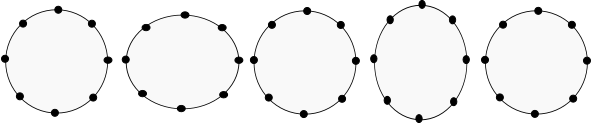
\includegraphics[width=0.5\linewidth]{img/RingOfParticles}
\end{tikzfigure}
}

\begin{wrapfigure}{r}{0.4\linewidth}
    \vspace{-10mm}
\begin{tikzfigure}
\centering
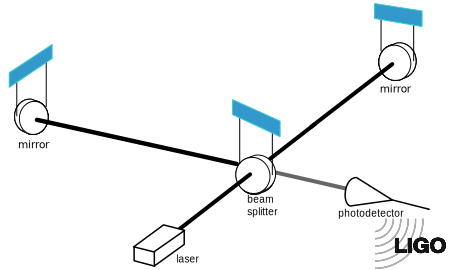
\includegraphics[width=\linewidth]{img/Ligo}
\end{tikzfigure}
\end{wrapfigure}

To detect gravitational waves we can use a laser interferometer. These split a
laser beam and send it off in two different directions; both beams are then
bounced off a mirror and return to the start. Both beams should have travelled
the same distance and so should return at the same time. However, if a
gravitational wave passed through during the experiment, they will not both
return at the same time. 

\end{minipage}
\hspace{5mm}
\vrule{}
\begin{minipage}[t]{0.44\linewidth}

The problem is that the differences between the two beams are very
small.  To put it in perspective, its like trying to measure that a human being
has grown by a single atom. We have built enourmous detectors in the hope of 
measuring gravitational waves, below is the 4 km long LIGO detector in the USA.
\begin{tikzfigure}
   \vspace{-8mm}
\centering
\includegraphics[width=.7\linewidth]{img/Hanford1_with_logo}
\end{tikzfigure}
Look out for results when the detectors turn on in 2016. 


\end{minipage}
}

\block[]{IV: Searching for signals from neutron stars}{

\begin{wrapfigure}{r}{0.33\linewidth}
    \vspace{-20mm}
\begin{tikzfigure}
\centering
\includegraphics[width=\linewidth]{img/CGW_example}
\end{tikzfigure}
\end{wrapfigure}

The signals we are searching for will be hidden in the  detector noise from seismic
activity and other sources. To search for it, we have to make a guess for what
the signal will look like, this is called a template. The template is then
compared to the data like in the graph on the right. This process relies on the
ability of the template to match the signal in the data. Using
the correct template is crucial to finding the signal.

Unfortunately it is possible that real gravitational wave signals will contain
noise from the neutron star itself.  This noise can look just like the detector
noise. I am trying to test how bad this effect will be and develop methods
to improve our chances of detection.

}

\begin{columns}

\column{0.5}
\block[]{V: Gravitational waves astronomy}{

Aside from testing Einsteins general relativity, gravitational waves will allow
us to explore the universe in a new way. Traditional astronomy observes
electromagnetic radiation from distant objects. This means we can only observe
the outside of hot, light emitting objects. With gravitational wave astronomy
we may be able to observe more of the many exotic and less explored areas
of physics 
such as black holes, neutron stars, and maybe even the big bang. 

}

\column{0.5}
\block[]{VI: Conclusions}{
\vspace{10mm}
    \centering
    \Large
We are trying to detect gravitational waves. Finding these is crucial evidence
for Einsteins theory of gravity, general relativity. If you
want to know more visit:

\vspace{7mm}
\centerline{
\textcolor{blue}{www.bit.do/LIGO}
}
\vspace{10mm}
}
\end{columns}

\end{document}



\endinput
%%
